\begin{pastexam}[label={px:ncku-113-prog-03}]{成大資訊聯招 113 學年度 第 3 題}
（單選）

\textbf{[2\%, 3\%]} Given a binary tree with the following postfix and infix patterns.
\begin{center}
\textit{postfix}: Z, P, C, L, Y, K, S, W, R, Q\\
\textit{infix}: Z, Y, P, L, C, Q, K, R, W, S
\end{center}
\begin{enumerate}[label=\roman*)]
\item What is the result of level-order traversal for the tree?

(A)~C, S, R, Z, L, K, W, Q, Y, P \qquad (B)~Q, Y, R, Z, L, K, W, P, C, S\\
(C)~Q, R, Y, W, K, L, Z, S, C, P \qquad (D)~Y, K, R, Z, Q, L, W, C, P, S\\
(E)~None of the above
\item What is the result of preorder traversal for the tree?

(A)~Q, Y, Z, L, P, C, R, K, W, S \qquad (B)~P, Z, C, Y, L, Q, K, R, W, S\\
(C)~Q, Y, Z, L, P, C, R, K, S, W \qquad (D)~P, Z, C, Y, L, Q, K, R, S, W\\
(E)~None of the above
\end{enumerate}
\end{pastexam}

\begin{pastsoln}
答案：i) (B)；ii) (A)。

\textbf{重建二元樹}（資結書第~7.4~節）。 後序的最後一個是根；在中序裡找到根，左邊是左子樹、右邊是
右子樹，兩段的長度也決定了後序怎麼切。 遞迴做下去：
\begin{center}
\small
\begin{tabular}{llll}
\toprule
子樹的後序 & 子樹的中序 & 根 & 左｜右（中序） \\
\midrule
Z P C L Y K S W R Q & Z Y P L C Q K R W S & Q & Z Y P L C ｜ K R W S \\
Z P C L Y & Z Y P L C & Y & Z ｜ P L C \\
P C L & P L C & L & P ｜ C \\
K S W R & K R W S & R & K ｜ W S \\
S W & W S & W & （空）｜ S \\
\bottomrule
\end{tabular}
\end{center}
（第一列：中序裡 Q 左邊有 $5$ 個，所以後序的前 $5$ 個 Z P C L Y 是左子樹，接著 K S W R 是右子樹。
最後一列：中序 W S 裡 W 在最前面，W 沒有左子樹，S 是它的右子節點。）
\begin{center}
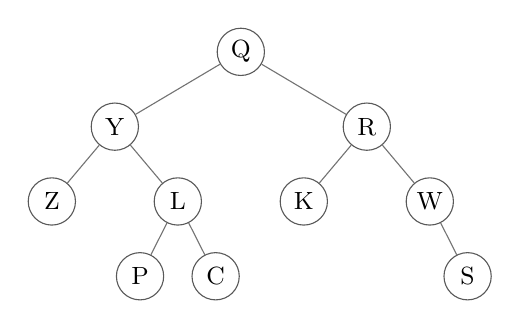
\begin{tikzpicture}[x=0.8cm,y=0.95cm,
  bn/.style={circle, draw=black!65, minimum size=0.6cm, inner sep=0pt, font=\small},
  be/.style={draw=black!55}]
\node[bn] (Q) at (4,0) {Q};
\node[bn] (Y) at (2,-1) {Y};
\node[bn] (R) at (6,-1) {R};
\node[bn] (Z) at (1,-2) {Z};
\node[bn] (L) at (3,-2) {L};
\node[bn] (K) at (5,-2) {K};
\node[bn] (W) at (7,-2) {W};
\node[bn] (P) at (2.4,-3) {P};
\node[bn] (C) at (3.6,-3) {C};
\node[bn] (S) at (7.6,-3) {S};
\draw[be] (Q)--(Y) (Q)--(R) (Y)--(Z) (Y)--(L) (L)--(P) (L)--(C) (R)--(K) (R)--(W) (W)--(S);
\end{tikzpicture}
\end{center}
檢查：這棵樹的中序是 Z, Y, P, L, C, Q, K, R, W, S，後序是 Z, P, C, L, Y, K, S, W, R, Q，都和題目一致。

i) 層序一層一層由左到右：第 1 層 Q；第 2 層 Y, R；第 3 層 Z, L, K, W；第 4 層 P, C, S。 得
Q, Y, R, Z, L, K, W, P, C, S，選 (B)。 (A)、(D) 第一個不是根 Q，錯；(C) 第 2 層把 R 放在 Y 前面，
左右顛倒，錯。

ii) 前序（根、左、右）：Q，左子樹 Y, Z, L, P, C，右子樹 R, K, W, S，得
Q, Y, Z, L, P, C, R, K, W, S，選 (A)。 (B)、(D) 第一個不是根，錯；(C) 最後是 S, W，但 W 是 S 的
父節點，前序要先 W 後 S，錯。
\end{pastsoln}
